
\section{Little Harder}

\subsection{If statements}
\begin{frame}[fragile]{Changing the Flow of Execution}
\begin{itemize}
\item Lets say we want to create a program that accepts a password. It only lets a user in \emph{if} their password is correct. For this we need an \emph{if}-statement.
\item \emph{if} statements use boolean values to decide whether or not to execute a \emph{block} of code.
\item Example:
\begin{semiverbatim}\code{
boolean allowed = false;
if ( allowed ) \{
    System.out.println("Hello World!"); \}
}\end{semiverbatim}
\item A \emph{block} is a \code{\texttt{\{}} followed by any number of \emph{statements} followed by a \code{\texttt{\}}}.
\item If a block does not follow an if statement then it decides whether or not to execute the next line of code.
\end{itemize}
\end{frame}

\begin{frame}[fragile]{Boolean Operators}

\begin{semiverbatim}\code{
boolean b = true \&\& true; \pause
b = true \&\& false; \pause
b = false \&\& false; \pause
b = true || true; \pause
b = true || false; \pause
b = false || false; \pause
b = !true; \pause
String s = "password";
if(s.equals("password"))\{
    b = (!false) \&\& true;
\}\pause else \{
    b = false;
\}
}\end{semiverbatim}
\end{frame}

\begin{frame}{A Few Things about Printing}
\begin{itemize}
\item We have been using \texttt{\code{System.out.println(<text>)}}. This prints the text to the console and then puts in a new line.
\item However we could use \texttt{\code{System.out.print(<text>)}}. This prints the text to the console, without putting in a new line. \pause
\item In addition to this there are a number of special characters you can use in a \emph{String}:
\begin{itemize}
\item {\textbackslash}t : tab.
\item {\textbackslash}n : newline.
\item {\textbackslash}{\textbackslash} : backslash.
\item {\textbackslash}b : backspace.
\item {\textbackslash}\texttt{"} : double quote.
\item {\textbackslash}\texttt{'} : quote.
\end{itemize}
\end{itemize}
\end{frame}

\begin{frame}{Harder Hello World}

\begin{center}
Extend Hello World so that it only prints if it receives the correct password from the user. The password should be passed as an \emph{argument} on the command line.
\end{center}
\end{frame}

\begin{frame}[fragile]{Example Code}
\begin{semiverbatim}\code{
public class HelloFinal \{
   public static void main(String[] args) \{
       if(args.length == 1) \{
          System.out.print("Hello ");
          System.out.print(args[0]);
          System.out.println("!");
       \}
       else \{
           System.out.println("Hello World!");
       \}
    \}
\}
}\end{semiverbatim}

\end{frame}

\subsection{Final HelloWorld!}
\begin{frame}[fragile]{The Scanner Class}
\begin{itemize}
\item While a program is running, we can get input from her by using the Scanner class. \pause
\item But first we must import the Scanner class.
\end{itemize}
\begin{semiverbatim}\code{
import java.util.Scanner;

public class Calculator
\{
}\end{semiverbatim}

$\vdots$
\end{frame}

\begin{frame}{What does import do?}
\begin{itemize}
\item What is this import thing!?! \pause
\item The \emph{import} statement tells the compiler where to look names, like Scanner. \pause
\item Instead of writing out \code{java.util.Scanner} every time we want to use the Scanner we can just use \code{Scanner} instead. \pause
\item We could also use \code{import java.util.\textsuperscript{*};} This imports everything from the \code{util} \emph{package}.
\item A \emph{package} is a folder that contains several classes.
\end{itemize}
\end{frame}

\begin{frame}[fragile]{Great so how do we use it?}
\begin{semiverbatim}\code{
import java.util.Scanner;

public class HW1
\{
   public static void main(String[] args)
   \{
      Scanner input = new Scanner(System.in);
      System.out.print("What is your name?");
      String name = input.next();
      System.out.print("What is your age?");
      int i = input.nextInt(); \pause
      double d = input.nextDouble(); \pause
      input.close();
}
\end{semiverbatim}
\end{frame}

\begin{frame}{Pop Quiz! Vocab edition!}
Give a short definition of the following:

\begin{itemize}
\item int \pause
\item double \pause
\item String \pause
\item char \pause
\item boolean \pause
\item package \pause
\item import statement \pause
\item operation \pause
\item if statement \pause
\item block \pause
\item argument \pause
\item statement
\end{itemize}

\end{frame}



\begin{frame}{Optional Activity}
\begin{center}
Using if statements and the Scanner class create a calculator in java. The calculator should ask the user what operation she wants to do, and then it should ask for two numbers. After the user puts in this information, the calculator prints out the answer.
\end{center}

\end{frame}

\begin{frame}{Begin the RPG}
\begin{center}
Using if statements and the Scanner class create a command line adventure game! This can be either a story where the player is given optional choices that affect the outcome or the player can battle a monster! If you finished the calculator exercise, you can reuse that code for this exercise.
\end{center}

\end{frame}



\section{Bonus and a lil' Homework}

\subsection{How does one install Java?}
\begin{frame}{Installing Java (Windows Instructions)}
\begin{itemize}
\item Java can also be installed on iOS and Java. Installation is more or less the same, if not easier than in Windows.
\item These instructions were made as of July 2014 for Windows 7. Modifications may be necessary for the future or for other operating systems.
\end{itemize}
\end{frame}

\begin{frame}{Where is Java?}
\begin{itemize}
\item To get the latest version of java, google ``java jdk." Click the first result. For me the site was:

    \begin{center}
    http://www.oracle.com/technetwork/java/javase\\
    /downloads/index.html
    \end{center}

\item Click JDK (Download). \\
\emph{What is this Netbeans thing? Do I need it? Net beans is an IDE that makes it easier to program. For this class we will be using a different IDE called Eclipse. Downloading it won't hurt, but you might not use it.}
\item Accept the user agreement, then download the correct distribution for your OS. \emph{x64 is for 64 bit OS's, while x86 is for 32 bit OS's.}
\end{itemize}
\end{frame}

\begin{frame}{What it Looked Like for Me}
\begin{center}
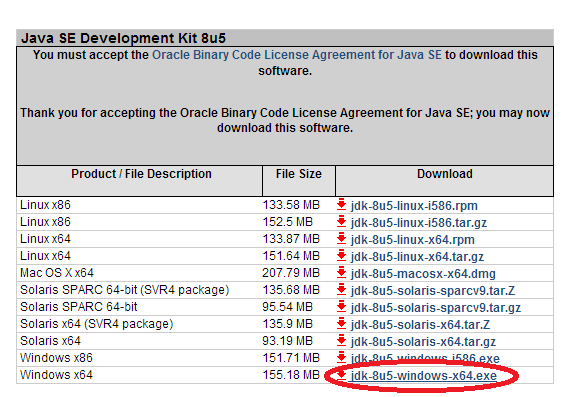
\includegraphics[width = 8cm]{Install1}
\end{center}
\end{frame}

\begin{frame}{Click next$\rightarrow$next$\rightarrow$ok$\rightarrow$next}
\begin{center}
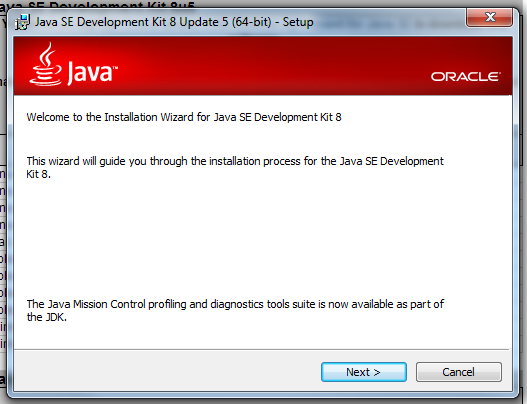
\includegraphics[width = 8cm]{Install2}
\end{center}
\end{frame}

\begin{frame}{Changing the PATH variable}
\begin{itemize}
\item Unfortunately we are not done.
\item Find the location of the binaries, kept in the \emph{bin} folder of the jdk. For example:
    \begin{center}C:{\textbackslash}Program Files{\textbackslash}Java{\textbackslash}jdk1.8.0\_05{\textbackslash}bin
    \end{center}

\item Go to Control Panel$\rightarrow$System and Security$\rightarrow$System$\rightarrow$Advanced System Settings$\rightarrow$(Advanced Tab)$\rightarrow$Environment Variables.
\item Click Path$\rightarrow$Edit
\end{itemize}
\end{frame}


\begin{frame}{The Important Step!!!}
\begin{itemize}
\item DO NOT DELETE the content next to ``Variable value".
\item Instead append a semicolon and then the location to the end of the variables. For example:

    \begin{itemize}
    \item Before: \code{$\ldots${\textbackslash}Windows Performance Toolkit{\textbackslash};C:{\textbackslash}Program Files{\textbackslash}Microsoft SQL Server{\textbackslash}110{\textbackslash}Tools{\textbackslash}Binn{\textbackslash}}
    \item After: \code{$\ldots${\textbackslash}Windows Performance Toolkit{\textbackslash};C:{\textbackslash}Program Files{\textbackslash}Microsoft SQL Server{\textbackslash}110{\textbackslash}Tools{\textbackslash}Binn{\textbackslash}\emph{\textbf{;}}C:{\textbackslash}Program Files{\textbackslash}Java{\textbackslash}jdk1.8.0\_05{\textbackslash}bin)}
    \end{itemize}
\end{itemize}
\end{frame}

\begin{frame}[fragile]{Testing}
\begin{itemize}
\item To test the correct installation run the following in the Command Prompt:
\begin{semiverbatim}\code{
C:{\textbackslash}Users{\textbackslash}Admin> javac -version
javac 1.8.0\_05

C:{\textbackslash}Users{\textbackslash}Admin>
}\end{semiverbatim}

\end{itemize}

\end{frame}

\begin{frame}{Some Screenshots}
\begin{center}
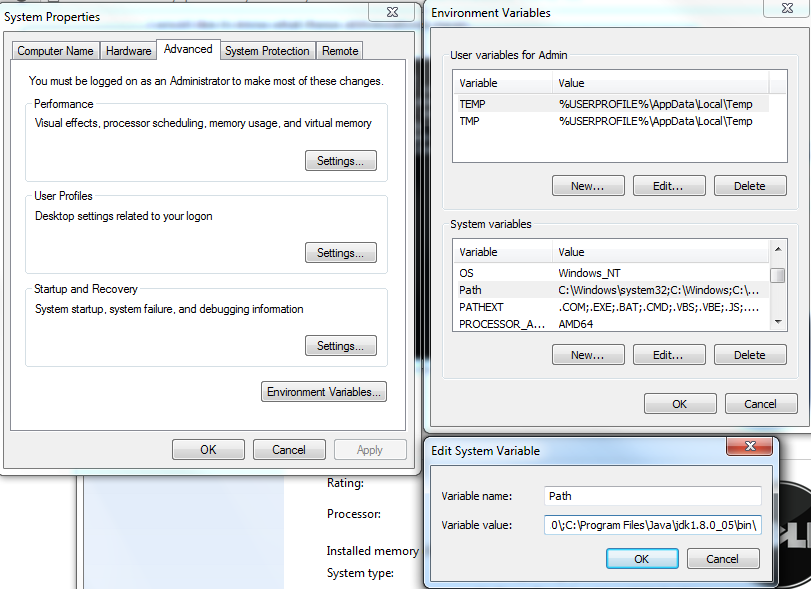
\includegraphics[width = 8cm]{Install3}
\end{center}
\end{frame}



\subsection{Homework Policy =(}
\begin{frame}{HW sometimes isn't fun, but this HW will be!}
\begin{center}
The homework is meant to help you remember and retain the information you learn the day you are in class. We will go over the answers the next day. The only policy is you must follow the directions, including spending no more than one hour on the homework! If it's not done that's ok, but try your best.
\end{center}

\end{frame}